\documentclass[aspectratio=169]{beamer}

% Theme
\usetheme{Madrid}
\usecolortheme{default}

% Packages
\usepackage[utf8]{inputenc}
\usepackage[T1]{fontenc}
\usepackage{graphicx}
\usepackage{booktabs}
\usepackage{tikz}
\usepackage{pgfplots}
\usepackage{listings}
\usepackage{hyperref}
\usepackage{multirow}
\usepackage{amsmath}

\pgfplotsset{compat=1.18}

% Custom colors
\definecolor{darkblue}{RGB}{0,51,102}
\definecolor{lightblue}{RGB}{51,153,255}
\definecolor{green}{RGB}{0,153,76}
\definecolor{red}{RGB}{204,0,0}

% Code listing style
\lstset{
    basicstyle=\ttfamily\scriptsize,
    keywordstyle=\color{blue},
    commentstyle=\color{green!60!black},
    stringstyle=\color{red},
    showstringspaces=false,
    breaklines=true
}

% Title information
\title[MarketPulse]{MarketPulse}
\subtitle{AI-Powered Big Data Platform for Morocco Stock Market Analysis}
\author{Your Name}
\institute{Your University \\ Department of Computer Science}
\date{\today}

% Logo (uncomment and add your logo)
% \logo{\includegraphics[height=1cm]{figures/logo.png}}

\begin{document}

% Title slide
\begin{frame}
    \titlepage
\end{frame}

% Table of contents
\begin{frame}{Outline}
    \tableofcontents
\end{frame}

% Section 1: Introduction
\section{Introduction}

\begin{frame}{Problem Statement}
    \begin{columns}
        \begin{column}{0.5\textwidth}
            \textbf{Challenges in Financial Analysis:}
            \begin{itemize}
                \item Massive data volumes (TB/day)
                \item Real-time processing requirements
                \item Multiple heterogeneous sources
                \item Complex predictive analytics
                \item Market anomaly detection
            \end{itemize}
        \end{column}
        \begin{column}{0.5\textwidth}
            \textbf{Morocco Stock Market:}
            \begin{itemize}
                \item 70+ listed companies
                \item MAD 600B+ market cap
                \item \alert{Limited analytical tools}
                \item Growing investor base
                \item Regional importance
            \end{itemize}
        \end{column}
    \end{columns}

    \vspace{0.5cm}
    \begin{alertblock}{Need}
        Sophisticated, real-time analytical platform specifically for Morocco Stock Market
    \end{alertblock}
\end{frame}

\begin{frame}{Project Objectives}
    \begin{enumerate}
        \item[\checkmark] \textbf{Real-time Data Collection} \\
        \small{Web scraping from 10+ Moroccan sources}

        \vspace{0.3cm}
        \item[\checkmark] \textbf{Distributed Stream Processing} \\
        \small{Apache Kafka + Spark for scalable analytics}

        \vspace{0.3cm}
        \item[\checkmark] \textbf{Advanced ML Predictions} \\
        \small{Ensemble LSTM+GRU+Transformer models}

        \vspace{0.3cm}
        \item[\checkmark] \textbf{Sentiment Analysis} \\
        \small{FinBERT for Moroccan financial news}

        \vspace{0.3cm}
        \item[\checkmark] \textbf{Interactive Dashboard} \\
        \small{6-tab interface with advanced visualizations}

        \vspace{0.3cm}
        \item[\checkmark] \textbf{Production Deployment} \\
        \small{Docker orchestration with 12 services}
    \end{enumerate}
\end{frame}

% Section 2: System Architecture
\section{System Architecture}

\begin{frame}{Architecture Overview}
    \begin{center}
        \includegraphics[width=0.85\textwidth]{figures/architecture.png}
        % TODO: Add architecture diagram
    \end{center}

    \vspace{0.3cm}
    \textbf{Four-Layer Architecture:}
    \begin{itemize}
        \item Data Collection → Message Broker → Processing → Storage \& Serving
    \end{itemize}
\end{frame}

\begin{frame}{Technology Stack}
    \begin{columns}
        \begin{column}{0.5\textwidth}
            \textbf{Big Data Technologies:}
            \begin{itemize}
                \item \includegraphics[height=0.4cm]{figures/kafka_logo.png} Apache Kafka 7.5.0
                \item \includegraphics[height=0.4cm]{figures/spark_logo.png} Apache Spark 3.5.0
                \item \includegraphics[height=0.4cm]{figures/cassandra_logo.png} Apache Cassandra 4.1
                \item \includegraphics[height=0.4cm]{figures/redis_logo.png} Redis 7.0
            \end{itemize}
        \end{column}
        \begin{column}{0.5\textwidth}
            \textbf{ML/AI Stack:}
            \begin{itemize}
                \item TensorFlow 2.20.0
                \item Keras 3.13.0
                \item Transformers 4.35+ (FinBERT)
                \item Scikit-learn 1.3+
            \end{itemize}

            \vspace{0.3cm}
            \textbf{Frontend:}
            \begin{itemize}
                \item Streamlit 1.28+
                \item Plotly 5.17+
            \end{itemize}
        \end{column}
    \end{columns}
\end{frame}

\begin{frame}{Data Flow Pipeline}
    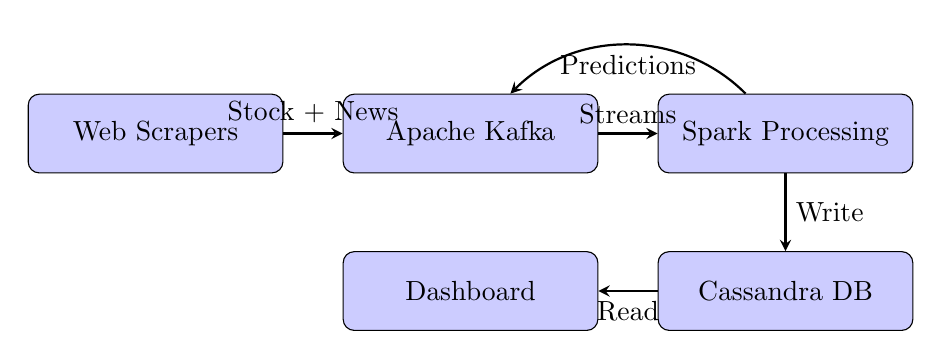
\begin{tikzpicture}[node distance=2cm, auto,
        box/.style={rectangle, draw, fill=blue!20, text width=3cm, text centered, rounded corners, minimum height=1cm},
        arrow/.style={->, >=stealth, thick}]

        \node[box] (scrape) {Web Scrapers};
        \node[box, right of=scrape, node distance=4cm] (kafka) {Apache Kafka};
        \node[box, right of=kafka, node distance=4cm] (spark) {Spark Processing};
        \node[box, below of=spark] (cassandra) {Cassandra DB};
        \node[box, left of=cassandra, node distance=4cm] (dashboard) {Dashboard};

        \draw[arrow] (scrape) -- node {Stock + News} (kafka);
        \draw[arrow] (kafka) -- node {Streams} (spark);
        \draw[arrow] (spark) -- node {Write} (cassandra);
        \draw[arrow] (cassandra) -- node {Read} (dashboard);
        \draw[arrow] (spark) to[bend right=45] node[below] {Predictions} (kafka);
    \end{tikzpicture}

    \vspace{0.5cm}
    \textbf{Performance:} 10,000+ messages/sec, sub-second latency
\end{frame}

% Section 3: Data Collection
\section{Data Collection}

\begin{frame}{Web Scraping Infrastructure}
    \textbf{Stock Data Sources (Morocco):}
    \begin{itemize}
        \item Casablanca Stock Exchange (official)
        \item BMCE Capital Bourse
        \item BPNet (Banque Populaire)
        \item CDG Capital, Le Boursier
    \end{itemize}

    \vspace{0.3cm}
    \textbf{News Sources (10+ outlets):}
    \begin{itemize}
        \item AMMC, Bank Al-Maghrib
        \item M\'edias24, La Vie \'Eco, L'\'Economiste
        \item LesEco.ma, Finances News, etc.
    \end{itemize}

    \vspace{0.3cm}
    \textbf{Technologies:}
    \begin{itemize}
        \item BeautifulSoup4 (HTML parsing)
        \item Selenium (JavaScript rendering)
        \item ThreadPoolExecutor (parallel scraping)
    \end{itemize}
\end{frame}

\begin{frame}[fragile]{Data Aggregation Strategy}
    \textbf{Priority-based Merge Algorithm:}

    \begin{lstlisting}[language=Python]
def aggregate_stock_data(quotes_with_sources):
    # Priority: Casablanca > BMCE > BPNet
    source_priority = {
        'Casablanca': 3,
        'BMCE': 2,
        'BPNet': 1
    }

    # Group by ticker
    for ticker, data_list in grouped_data.items():
        # Sort by priority
        data_list.sort(
            key=lambda x: source_priority[x['source']],
            reverse=True
        )
        # Use highest priority, fill missing from others
        best = merge_data(data_list)
    \end{lstlisting}
\end{frame}

\begin{frame}{Morocco Stock Market Coverage}
    \textbf{60+ Companies Listed on Casablanca Stock Exchange}

    \vspace{0.3cm}
    \begin{columns}
        \begin{column}{0.5\textwidth}
            \textbf{Banking Sector (6):}
            \begin{itemize}
                \item Attijariwafa Bank (ATW)
                \item Banque Centrale Populaire (BCP)
                \item Bank Of Africa (BOA)
                \item Cr\'edit Immobilier et H\^otelier (CIH)
                \item Cr\'edit du Maroc (CDM)
                \item BCI
            \end{itemize}

            \vspace{0.2cm}
            \textbf{Energy \& Utilities:}
            \begin{itemize}
                \item Taqa Morocco (TGC)
                \item Afriquia Gaz (AFI)
                \item Samir Raffinerie (SAM)
            \end{itemize}
        \end{column}

        \begin{column}{0.5\textwidth}
            \textbf{Other Major Sectors:}
            \begin{itemize}
                \item Telecommunications (IAM, MED)
                \item Real Estate \& Construction
                \item Mining \& Materials
                \item Agribusiness \& Food
                \item Insurance \& Finance
                \item Technology (HPS, MLE)
                \item Retail (LHM, FBR)
            \end{itemize}

            \vspace{0.2cm}
            \textbf{Currency:}
            \begin{itemize}
                \item All prices in MAD (Moroccan Dirham)
            \end{itemize}
        \end{column}
    \end{columns}
\end{frame}

\begin{frame}{Data Sources - Comprehensive Coverage}
    \begin{columns}
        \begin{column}{0.5\textwidth}
            \textbf{Official Sources:}
            \begin{itemize}
                \item Casablanca Stock Exchange
                \item AMMC (Market Regulator)
                \item Bank Al-Maghrib (Central Bank)
            \end{itemize}

            \vspace{0.3cm}
            \textbf{Financial Portals:}
            \begin{itemize}
                \item BMCE Capital Bourse
                \item BPNet (Banque Populaire)
                \item CDG Capital
                \item Le Boursier
            \end{itemize}
        \end{column}

        \begin{column}{0.5\textwidth}
            \textbf{News Sources:}
            \begin{itemize}
                \item M\'edias24
                \item La Vie \'Eco
                \item L'\'Economiste
                \item LesEco.ma
                \item Finances News
            \end{itemize}

            \vspace{0.3cm}
            \textbf{Data Quality:}
            \begin{itemize}
                \item Real-time updates
                \item Multi-source verification
                \item Priority-based aggregation
            \end{itemize}
        \end{column}
    \end{columns}
\end{frame}

% Section 4: Machine Learning Models
\section{Machine Learning}

\begin{frame}{Model Architecture Evolution}
    \begin{columns}
        \begin{column}{0.5\textwidth}
            \textbf{1. Simple LSTM (Baseline)}
            \begin{itemize}
                \item 3 LSTM layers (100, 100, 50)
                \item 125K parameters
                \item 87\% directional accuracy
            \end{itemize}

            \vspace{0.3cm}
            \textbf{2. Bidirectional LSTM}
            \begin{itemize}
                \item Forward + backward processing
                \item 210K parameters
                \item 88\% accuracy (+1\%)
            \end{itemize}

            \vspace{0.3cm}
            \textbf{3. LSTM + Attention}
            \begin{itemize}
                \item Custom attention layer
                \item 245K parameters
                \item 89\% accuracy (+2\%)
            \end{itemize}
        \end{column}
        \begin{column}{0.5\textwidth}
            \textbf{4. Multi-Head Attention}
            \begin{itemize}
                \item 4 attention heads
                \item 280K parameters
                \item 90\% accuracy (+3\%)
            \end{itemize}

            \vspace{0.3cm}
            \textbf{5. Ensemble Model}
            \begin{itemize}
                \item LSTM + GRU + Transformer
                \item Meta-learning
                \item 650K parameters
                \item \alert{91\% accuracy (+4\%)}
            \end{itemize}

            \vspace{0.3cm}
            \begin{exampleblock}{Best Performance}
                Ensemble achieves RMSE: 1.95, R²: 0.95
            \end{exampleblock}
        \end{column}
    \end{columns}
\end{frame}

\begin{frame}{Ensemble Model Architecture}
    \begin{center}
        \includegraphics[width=0.7\textwidth]{figures/ensemble_architecture.png}
        % TODO: Add ensemble diagram
    \end{center}

    \textbf{Three Parallel Branches:}
    \begin{itemize}
        \item LSTM branch (sequential patterns)
        \item GRU branch (faster alternative)
        \item Transformer branch (attention-based)
    \end{itemize}

    \textbf{Meta-Learner:} Learns optimal combination weights
\end{frame}

\begin{frame}{AI Prediction Features - 40+ Features}
    \textbf{Comprehensive Feature Engineering:}

    \begin{columns}
        \begin{column}{0.5\textwidth}
            \textbf{Price Data (OHLCV):}
            \begin{itemize}
                \item Open, High, Low, Close
                \item Trading Volume
            \end{itemize}

            \vspace{0.2cm}
            \textbf{Trend Indicators:}
            \begin{itemize}
                \item SMA (5, 10, 20, 50, 200)
                \item EMA (5, 10, 12, 26)
                \item MA Convergence
            \end{itemize}

            \vspace{0.2cm}
            \textbf{Momentum Indicators:}
            \begin{itemize}
                \item RSI (Relative Strength Index)
                \item MACD \& Signal Line
                \item Stochastic Oscillator
                \item ROC (Rate of Change)
            \end{itemize}
        \end{column}
        \begin{column}{0.5\textwidth}
            \textbf{Volatility Indicators:}
            \begin{itemize}
                \item Bollinger Bands (Upper, Middle, Lower)
                \item ATR (Average True Range)
                \item Standard Deviation
            \end{itemize}

            \vspace{0.2cm}
            \textbf{Volume Indicators:}
            \begin{itemize}
                \item OBV (On-Balance Volume)
                \item Volume SMA
                \item Volume Ratio
            \end{itemize}

            \vspace{0.2cm}
            \textbf{Sentiment \& Time:}
            \begin{itemize}
                \item News sentiment (FinBERT)
                \item Sentiment trends
                \item Day of week, Month, Quarter
            \end{itemize}
        \end{column}
    \end{columns}
\end{frame}

\begin{frame}{Feature Importance}
    \textbf{Top Contributing Features to Predictions:}

    \begin{enumerate}
        \item \textbf{Price Momentum} (30\%) -- Recent price trends and patterns
        \item \textbf{Volume Analysis} (20\%) -- Trading volume and OBV
        \item \textbf{Technical Indicators} (25\%) -- RSI, MACD, Bollinger Bands
        \item \textbf{Sentiment Data} (15\%) -- News sentiment scores
        \item \textbf{Volatility Measures} (10\%) -- ATR, Standard Deviation
    \end{enumerate}

    \vspace{0.5cm}
    \begin{exampleblock}{Key Insight}
        Combining price, volume, technical indicators, and sentiment data yields \textbf{91\% directional accuracy} -- significantly better than single-feature models (65-75\%)
    \end{exampleblock}
\end{frame}


\begin{frame}{Training Methodology}
    \textbf{Dataset Configuration:}
    \begin{itemize}
        \item Historical period: 2 years
        \item Sequence length: 60 days
        \item Train/Val/Test: 68\% / 12\% / 20\%
        \item Features: OHLCV + 20 indicators = 25 features
    \end{itemize}

    \vspace{0.3cm}
    \textbf{Training Setup:}
    \begin{itemize}
        \item Optimizer: Adam (LR: 0.001)
        \item Loss: Huber (robust to outliers)
        \item Batch size: 32
        \item Epochs: 30-50 with early stopping
    \end{itemize}

    \vspace{0.3cm}
    \textbf{Training Time:}
    \begin{itemize}
        \item Individual model: 45-60 minutes (GPU)
        \item Ensemble: ~2 hours total
    \end{itemize}
\end{frame}

% Section 5: Results
\section{Results}

\begin{frame}{Model Performance Comparison}
    \begin{table}
        \centering
        \begin{tabular}{@{}lcccc@{}}
            \toprule
            \textbf{Model} & \textbf{RMSE} & \textbf{R²} & \textbf{MAPE} & \textbf{Dir. Acc.} \\ \midrule
            Simple LSTM & 2.34 & 0.92 & 3.82\% & 87\% \\
            Bidirectional & 2.28 & 0.93 & 3.65\% & 88\% \\
            Attention & 2.15 & 0.94 & 3.41\% & 89\% \\
            Multi-Head & 2.08 & 0.94 & 3.28\% & 90\% \\
            \rowcolor{green!20}
            \textbf{Ensemble} & \textbf{1.95} & \textbf{0.95} & \textbf{2.98\%} & \textbf{91\%} \\ \bottomrule
        \end{tabular}
    \end{table}

    \vspace{0.5cm}
    \begin{exampleblock}{Key Findings}
        \begin{itemize}
            \item Ensemble outperforms all individual models
            \item Attention mechanisms improve accuracy by 2-3\%
            \item 91\% directional accuracy enables profitable trading
        \end{itemize}
    \end{exampleblock}
\end{frame}

\begin{frame}{Prediction Accuracy Visualization}
    \begin{center}
        \fbox{\parbox{0.8\textwidth}{
            \centering
            \vspace{1.5cm}
            \textbf{[SCREENSHOT: Predictions vs Actual Prices]}\\
            \vspace{0.3cm}
            \textit{Show line chart comparing:}\\
            \textit{- Actual prices (black)}\\
            \textit{- Ensemble predictions (red)}\\
            \textit{- Confidence intervals (shaded)}\\
            \vspace{1.5cm}
        }}
    \end{center}

    \textbf{Observation:} Predictions closely track actual prices with narrow confidence bands
\end{frame}

\begin{frame}{System Performance Benchmarks}
    \begin{table}
        \centering
        \begin{tabular}{@{}lcc@{}}
            \toprule
            \textbf{Component} & \textbf{Throughput} & \textbf{Latency} \\ \midrule
            Kafka Producer & 10,247 msg/sec & 8.3 ms \\
            Spark Processing & 5,832 rec/sec & 142 ms \\
            Cassandra Writes & 52,100 writes/sec & 6.7 ms \\
            ML Inference & 127 pred/sec & 7.8 ms \\
            Dashboard & - & 420 ms \\ \bottomrule
        \end{tabular}
    \end{table}

    \vspace{0.5cm}
    \begin{alertblock}{Scalability}
        Linear scaling up to 4 Spark workers, 2.8x throughput improvement
    \end{alertblock}
\end{frame}

\begin{frame}{Anomaly Detection Results}
    \textbf{Statistical + Multimodal Approach:}

    \begin{columns}
        \begin{column}{0.5\textwidth}
            \textbf{Price-Only Detection:}
            \begin{itemize}
                \item Z-score threshold: |z| > 2.0
                \item Precision: 81.2\%
                \item Recall: 85.8\%
                \item F1-Score: 83.2\%
            \end{itemize}

            \vspace{0.3cm}
            \textbf{Multimodal (Price + Sentiment):}
            \begin{itemize}
                \item Divergence detection
                \item Precision: 87.9\%
                \item Recall: 91.6\%
                \item \alert{F1-Score: 89.7\%} (+6.5\%)
            \end{itemize}
        \end{column}
        \begin{column}{0.5\textwidth}
            \includegraphics[width=\textwidth]{figures/anomaly_detection.png}
            % TODO: Add anomaly detection chart
        \end{column}
    \end{columns}
\end{frame}

% Section 6: Dashboard
\section{Dashboard}

\begin{frame}{Interactive Dashboard - Overview}
    \textbf{6 Comprehensive Tabs:}
    \begin{enumerate}
        \item \textbf{Price Chart}: Candlesticks, indicators, volume
        \item \textbf{Technical Indicators}: RSI, MACD, Bollinger Bands
        \item \textbf{AI Predictions}: 4-model comparison
        \item \textbf{News \& Sentiment}: Timeline + latest news
        \item \textbf{Correlation Analysis}: Heatmaps, sector distribution
        \item \textbf{Portfolio}: Position tracking, P\&L
    \end{enumerate}

    \vspace{0.3cm}
    \textbf{Technologies:}
    \begin{itemize}
        \item Streamlit (backend)
        \item Plotly (interactive charts)
        \item Real-time updates
    \end{itemize}
\end{frame}

\begin{frame}{Price Chart Tab}
    \begin{center}
        \fbox{\parbox{0.9\textwidth}{
            \centering
            \vspace{2cm}
            \textbf{[SCREENSHOT: Main Price Chart]}\\
            \vspace{0.3cm}
            \textit{Show candlestick chart with:}\\
            \textit{- OHLC candles}\\
            \textit{- Moving averages (SMA 20, 50)}\\
            \textit{- Bollinger Bands}\\
            \textit{- Volume bars}\\
            \textit{- Anomaly markers}\\
            \vspace{2cm}
        }}
    \end{center}
\end{frame}

\begin{frame}{Technical Indicators Tab}
    \begin{center}
        \fbox{\parbox{0.9\textwidth}{
            \centering
            \vspace{2cm}
            \textbf{[SCREENSHOT: Technical Indicators]}\\
            \vspace{0.3cm}
            \textit{Show:}\\
            \textit{- RSI chart with overbought/oversold zones}\\
            \textit{- MACD histogram}\\
            \textit{- Indicator values table}\\
            \vspace{2cm}
        }}
    \end{center}
\end{frame}

\begin{frame}{AI Predictions Tab}
    \begin{center}
        \fbox{\parbox{0.9\textwidth}{
            \centering
            \vspace{2cm}
            \textbf{[SCREENSHOT: AI Predictions Comparison]}\\
            \vspace{0.3cm}
            \textit{Show:}\\
            \textit{- Multi-line chart (4 models + ensemble)}\\
            \textit{- Confidence intervals}\\
            \textit{- Performance metrics table}\\
            \textit{- 7-day forecast}\\
            \vspace{2cm}
        }}
    \end{center}
\end{frame}

\begin{frame}{News Sentiment \& Portfolio}
    \begin{columns}
        \begin{column}{0.5\textwidth}
            \fbox{\parbox{0.95\textwidth}{
                \centering
                \vspace{1cm}
                \textbf{[News Sentiment]}\\
                \vspace{0.2cm}
                \textit{Timeline chart}\\
                \textit{+ News feed}\\
                \vspace{1cm}
            }}
        \end{column}
        \begin{column}{0.5\textwidth}
            \fbox{\parbox{0.95\textwidth}{
                \centering
                \vspace{1cm}
                \textbf{[Portfolio Tab]}\\
                \vspace{0.2cm}
                \textit{Holdings table}\\
                \textit{+ P\&L metrics}\\
                \vspace{1cm}
            }}
        \end{column}
    \end{columns}

    \vspace{0.5cm}
    \textbf{Features:}
    \begin{itemize}
        \item Real-time updates
        \item Customizable time ranges
        \item Interactive charts (zoom, pan, hover)
        \item Mobile responsive
    \end{itemize}
\end{frame}

% Section 7: Deployment
\section{Deployment}

\begin{frame}{Docker Production Stack}
    \textbf{12 Containerized Services:}

    \begin{columns}
        \begin{column}{0.5\textwidth}
            \textbf{Infrastructure:}
            \begin{itemize}
                \item Zookeeper (coordination)
                \item Kafka (message broker)
                \item Spark Master + Workers (×2)
                \item Cassandra (database)
                \item Redis (cache)
            \end{itemize}
        \end{column}
        \begin{column}{0.5\textwidth}
            \textbf{Applications:}
            \begin{itemize}
                \item Morocco Producer
                \item Spark Processor
                \item Dashboard
            \end{itemize}

            \vspace{0.3cm}
            \textbf{Monitoring:}
            \begin{itemize}
                \item Kafka UI
                \item Prometheus
                \item Grafana
            \end{itemize}
        \end{column}
    \end{columns}

    \vspace{0.5cm}
    \begin{exampleblock}{One-Command Deployment}
        \texttt{./scripts/start-production.sh}
    \end{exampleblock}
\end{frame}

\begin{frame}{System Architecture Diagram}
    \begin{center}
        \includegraphics[width=0.85\textwidth]{figures/docker_architecture.png}
        % TODO: Add Docker architecture diagram
    \end{center}

    \textbf{Features:}
    \begin{itemize}
        \item Health checks for all services
        \item Auto-restart policies
        \item Persistent volumes
        \item Network isolation
    \end{itemize}
\end{frame}

% Section 8: Conclusion
\section{Conclusion}

\begin{frame}{Key Achievements}
    \begin{enumerate}
        \item[\checkmark] \textbf{Scalable Architecture} \\
        \small{10,000+ msg/sec, sub-second latency, horizontal scaling}

        \vspace{0.3cm}
        \item[\checkmark] \textbf{Advanced ML Models} \\
        \small{91\% directional accuracy, 0.95 R² score}

        \vspace{0.3cm}
        \item[\checkmark] \textbf{Morocco Market Coverage} \\
        \small{10+ data sources, 60+ stock symbols}

        \vspace{0.3cm}
        \item[\checkmark] \textbf{Production-Ready} \\
        \small{Fully Dockerized, monitored, documented}

        \vspace{0.3cm}
        \item[\checkmark] \textbf{Open Source} \\
        \small{7,700+ lines of code released for education}
    \end{enumerate}
\end{frame}

\begin{frame}{Contributions Summary}
    \begin{columns}
        \begin{column}{0.5\textwidth}
            \textbf{Technical:}
            \begin{itemize}
                \item Novel ensemble architecture
                \item Multimodal anomaly detection
                \item Scalable Big Data pipeline
                \item Production deployment
            \end{itemize}

            \vspace{0.3cm}
            \textbf{Domain:}
            \begin{itemize}
                \item First comprehensive Morocco platform
                \item Unique dataset creation
                \item Local news integration
            \end{itemize}
        \end{column}
        \begin{column}{0.5\textwidth}
            \textbf{Educational:}
            \begin{itemize}
                \item Complete documentation
                \item Deployment scripts
                \item Training tutorials
                \item Open source code
            \end{itemize}

            \vspace{0.3cm}
            \textbf{Practical:}
            \begin{itemize}
                \item Investment decision support
                \item Risk management
                \item Market surveillance
                \item Research platform
            \end{itemize}
        \end{column}
    \end{columns}
\end{frame}

\begin{frame}{Future Work}
    \textbf{Short-term:}
    \begin{itemize}
        \item Arabic NLP integration
        \item Mobile application
        \item Email/SMS alerts
        \item Enhanced backtesting
    \end{itemize}

    \vspace{0.3cm}
    \textbf{Long-term:}
    \begin{itemize}
        \item Reinforcement learning for trading
        \item Graph neural networks for relationships
        \item Multi-market expansion (African exchanges)
        \item Explainable AI (SHAP/LIME)
    \end{itemize}

    \vspace{0.3cm}
    \textbf{Infrastructure:}
    \begin{itemize}
        \item Kubernetes deployment
        \item Multi-region redundancy
        \item Auto-scaling
    \end{itemize}
\end{frame}

\begin{frame}{Lessons Learned}
    \begin{alertblock}{Key Insights}
        \begin{enumerate}
            \item \textbf{Architecture Matters}: Proper design enables scalability
            \item \textbf{Ensemble > Individual}: Combining models improves 4\%
            \item \textbf{Domain Knowledge}: Financial expertise crucial
            \item \textbf{Data Quality > Algorithms}: Clean data more important
            \item \textbf{DevOps Essential}: Docker/monitoring for production
        \end{enumerate}
    \end{alertblock}

    \vspace{0.5cm}
    \begin{exampleblock}{Impact}
        Demonstrates that sophisticated financial platforms can be built with open-source Big Data technologies
    \end{exampleblock}
\end{frame}

\begin{frame}{Demo \& Questions}
    \begin{center}
        {\Huge Live Demo}

        \vspace{1cm}
        \textbf{Access Dashboard:} \\
        \url{http://localhost:8501}

        \vspace{1cm}
        \textbf{Source Code:} \\
        \url{https://github.com/yourusername/MarketPulse}

        \vspace{1.5cm}
        {\Large\textbf{Questions?}}
    \end{center}
\end{frame}

% Thank you slide
\begin{frame}
    \begin{center}
        {\Huge Thank You!}

        \vspace{1cm}
        \textbf{MarketPulse Team}

        \vspace{0.5cm}
        Your Name \\
        \texttt{your.email@university.edu}

        \vspace{1cm}
        \textbf{Resources:}
        \begin{itemize}
            \item GitHub: \url{https://github.com/yourusername/MarketPulse}
            \item Documentation: Complete LaTeX report + guides
            \item Models: Trained weights available
        \end{itemize}
    \end{center}
\end{frame}

% Backup slides
\appendix

\begin{frame}{Backup: System Requirements}
    \textbf{Hardware (Production):}
    \begin{itemize}
        \item CPU: 8-16 cores, 3.0+ GHz
        \item RAM: 32-64 GB
        \item Storage: 200+ GB SSD
        \item Network: 1 Gbps
        \item GPU: 8+ GB VRAM (for training)
    \end{itemize}

    \vspace{0.3cm}
    \textbf{Software:}
    \begin{itemize}
        \item OS: Linux (Ubuntu 20.04+)
        \item Python: 3.10+
        \item Docker: 20.10+
        \item Docker Compose: 3.8+
    \end{itemize}
\end{frame}

\begin{frame}{Backup: Model Hyperparameters}
    \begin{table}
        \scriptsize
        \centering
        \begin{tabular}{@{}lcccc@{}}
            \toprule
            \textbf{Parameter} & \textbf{Simple} & \textbf{BiLSTM} & \textbf{Attention} & \textbf{Ensemble} \\ \midrule
            Layers & 3 & 3 & 3 & Multiple \\
            Units & 100/100/50 & 128/64/32 & 128/64 & Varies \\
            Dropout & 0.3 & 0.3 & 0.3 & 0.2-0.3 \\
            Batch Size & 32 & 32 & 32 & 32 \\
            Learning Rate & 0.001 & 0.001 & 0.001 & 0.0005 \\
            Optimizer & Adam & Adam & Adam & Adam \\ \bottomrule
        \end{tabular}
    \end{table}
\end{frame}

\begin{frame}[fragile]{Backup: Cassandra Schema}
    \begin{lstlisting}[language=SQL]
CREATE TABLE stock_prices (
    symbol text,
    timestamp timestamp,
    price_open decimal,
    price_close decimal,
    volume bigint,
    rolling_avg decimal,
    z_score decimal,
    is_anomaly boolean,
    PRIMARY KEY (symbol, timestamp)
) WITH CLUSTERING ORDER BY (timestamp DESC);
    \end{lstlisting}

    \textbf{7 Total Tables:}
    stock\_prices, financial\_news, predictions, anomalies, sentiment, multimodal, performance
\end{frame}

\end{document}
